\documentclass{beamer}
\author{Shaun Schreiber (16715128)}
\title{Flow modelling and Cellular Automata}
\usetheme{Oxygen}
\usepackage{tikz,ifthen}
\date{\today}
\begin{document}
	\frame{\titlepage}
	%one
	\begin{frame}
	\frametitle{Outline}
    \tableofcontents[section=1,hidesubsections]
	\end{frame}

	%two
	\section{Lattice gas cellular automata}
	\begin{frame}
	\frametitle{Lattice gas cellular automata}
	\minipage{0.45\textwidth}
    \begin{block}{Difference}
  	\Large What is the difference between lattice gas cellular automata (LGCA) and CA?
  	\end{block}
  	\endminipage\hfill
	\minipage{0.45\textwidth}
    \begin{block}{Basic structure}
    \begin{figure}[H]
  \centering
  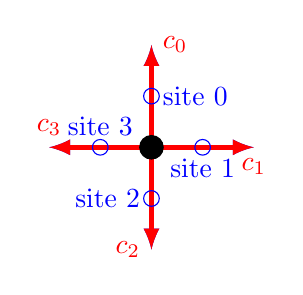
\begin{tikzpicture}[scale=0.65]

    \coordinate (Origin) at (0,0);
    \coordinate (site1) at (0,2);
    \coordinate (site2) at (2,0);
    \coordinate (site3) at (0,-2);
    \coordinate (site4) at (-2,0);  
    
    \draw [ultra thick,-latex,blue] (Origin)
        -- (site1) node [midway, right] {site 0};
    \draw [ultra thick,-latex,blue] (Origin)
        -- (site2) node [midway,below] {site 1};
    \draw [ultra thick,-latex,blue] (Origin)
        -- (site3) node [midway,left] {site 2};
    \draw [ultra thick,-latex,blue] (Origin)
        -- (site4) node [midway,above] {site 3};
        
	\draw [ultra thick,-latex,red] (Origin)
        -- (site1) node [right] {$c_0$};
    \draw [ultra thick,-latex,red] (Origin)
        -- (site2) node [below] {$c_1$};
    \draw [ultra thick,-latex,red] (Origin)
        -- (site3) node [left] {$c_2$};
    \draw [ultra thick,-latex,red] (Origin)
        -- (site4) node [above] {$c_3$};
       
    \node[draw,circle,inner sep=3pt,fill] at (0,0) {};
    \node[draw,circle,inner sep=2pt,blue] at (1,0) {};
	\node[draw,circle,inner sep=2pt,blue] at (0,1) {};
	\node[draw,circle,inner sep=2pt,blue] at (-1,0) {};
	\node[draw,circle,inner sep=2pt,blue] at (0,-1) {};
  \end{tikzpicture}
  \caption{Here is an example of a single cell with 4 velocity vectors and 4 empty sites.}
  \label{figure:single-cell}
\end{figure}
    \end{block}
    \endminipage\hfill

	\end{frame}

	%three
	\section{LGCA in flow modelling}
	\begin{frame}
	\frametitle{LGCA in flow modelling}
	\minipage{0.45\textwidth}
	\centering
    \begin{block}{Lattices Models}
    \begin{itemize}
    \item HPP 
    \item FHP
    \item LBM
    \end{itemize}
    \end{block}
    \endminipage\hfill
	\end{frame}

	%four
	\section{HPP}
	\begin{frame}
	\frametitle{HPP}
	\minipage{0.45\textwidth}
    \begin{block}{History}
	\begin{itemize}
    \item Developed in 1973.
    \item By Hardy, de Pazzis and Pomeau.
    \item Fail Navier-Stokes.
    \end{itemize}
    \end{block}
    \endminipage\hfill
    \minipage{0.45\textwidth}
    \begin{block}{One cell.}
\begin{figure}[H]
  \centering
  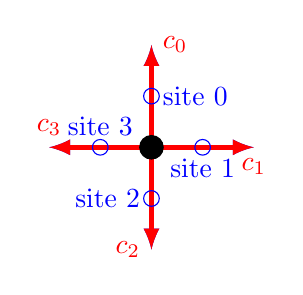
\begin{tikzpicture}[scale=0.65]

    \coordinate (Origin) at (0,0);
    \coordinate (site1) at (0,2);
    \coordinate (site2) at (2,0);
    \coordinate (site3) at (0,-2);
    \coordinate (site4) at (-2,0);  
    
    \draw [ultra thick,-latex,blue] (Origin)
        -- (site1) node [midway, right] {site 0};
    \draw [ultra thick,-latex,blue] (Origin)
        -- (site2) node [midway,below] {site 1};
    \draw [ultra thick,-latex,blue] (Origin)
        -- (site3) node [midway,left] {site 2};
    \draw [ultra thick,-latex,blue] (Origin)
        -- (site4) node [midway,above] {site 3};
        
	\draw [ultra thick,-latex,red] (Origin)
        -- (site1) node [right] {$c_0$};
    \draw [ultra thick,-latex,red] (Origin)
        -- (site2) node [below] {$c_1$};
    \draw [ultra thick,-latex,red] (Origin)
        -- (site3) node [left] {$c_2$};
    \draw [ultra thick,-latex,red] (Origin)
        -- (site4) node [above] {$c_3$};
       
    \node[draw,circle,inner sep=3pt,fill] at (0,0) {};
    \node[draw,circle,inner sep=2pt,blue] at (1,0) {};
	\node[draw,circle,inner sep=2pt,blue] at (0,1) {};
	\node[draw,circle,inner sep=2pt,blue] at (-1,0) {};
	\node[draw,circle,inner sep=2pt,blue] at (0,-1) {};
  \end{tikzpicture}
  \caption{Here is an example of a single cell with 4 velocity vectors and 4 empty sites.}
  \label{figure:single-cell}
\end{figure}
  	\end{block}
  	\endminipage\hfill
	\end{frame}

	%five
	\subsection{HPP Collision Phase}
	\begin{frame}
	\frametitle{HPP Collision Phase}
	\minipage{0.45\textwidth}
	\begin{block}{Before}
	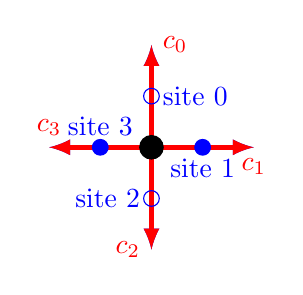
\begin{tikzpicture}[scale=0.65]
    \coordinate (Origin) at (0,0);
    \coordinate (site1) at (0,2);
    \coordinate (site2) at (2,0);
    \coordinate (site3) at (0,-2);
    \coordinate (site4) at (-2,0);  
    
    \draw [ultra thick,-latex,blue] (Origin)
        -- (site1) node [midway, right] {site 0};
    \draw [ultra thick,-latex,blue] (Origin)
        -- (site2) node [midway,below] {site 1};
    \draw [ultra thick,-latex,blue] (Origin)
        -- (site3) node [midway,left] {site 2};
    \draw [ultra thick,-latex,blue] (Origin)
        -- (site4) node [midway,above] {site 3};
        
	\draw [ultra thick,-latex,red] (Origin)
        -- (site1) node [right] {$c_0$};
    \draw [ultra thick,-latex,red] (Origin)
        -- (site2) node [below] {$c_1$};
    \draw [ultra thick,-latex,red] (Origin)
        -- (site3) node [left] {$c_2$};
    \draw [ultra thick,-latex,red] (Origin)
        -- (site4) node [above] {$c_3$};
       
    \node[draw,circle,inner sep=3pt,fill] at (0,0) {};
    \node[draw,circle,inner sep=2pt,fill,blue] at (1,0) {};
	\node[draw,circle,inner sep=2pt,blue] at (0,1) {};
	\node[draw,circle,inner sep=2pt,fill,blue] at (-1,0) {};
	\node[draw,circle,inner sep=2pt,blue] at (0,-1) {};
  \end{tikzpicture}
  \caption{Before Collision}
    \end{block}
    \endminipage\hfill
    \minipage{0.45\textwidth}
	\begin{block}{After}
	 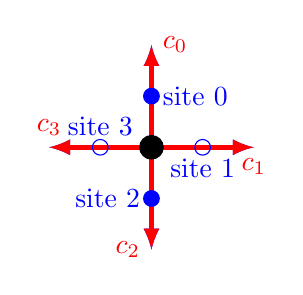
\begin{tikzpicture}[scale=0.65]
    \coordinate (Origin) at (0,0);
    \coordinate (site1) at (0,2);
    \coordinate (site2) at (2,0);
    \coordinate (site3) at (0,-2);
    \coordinate (site4) at (-2,0);  
    
    \draw [ultra thick,-latex,blue] (Origin)
        -- (site1) node [midway, right] {site 0};
    \draw [ultra thick,-latex,blue] (Origin)
        -- (site2) node [midway,below] {site 1};
    \draw [ultra thick,-latex,blue] (Origin)
        -- (site3) node [midway,left] {site 2};
    \draw [ultra thick,-latex,blue] (Origin)
        -- (site4) node [midway,above] {site 3};
        
	\draw [ultra thick,-latex,red] (Origin)
        -- (site1) node [right] {$c_0$};
    \draw [ultra thick,-latex,red] (Origin)
        -- (site2) node [below] {$c_1$};
    \draw [ultra thick,-latex,red] (Origin)
        -- (site3) node [left] {$c_2$};
    \draw [ultra thick,-latex,red] (Origin)
        -- (site4) node [above] {$c_3$};
       
    \node[draw,circle,inner sep=3pt,fill] at (0,0) {};
    \node[draw,circle,inner sep=2pt,blue] at (1,0) {};
	\node[draw,circle,inner sep=2pt,fill,blue] at (0,1) {};
	\node[draw,circle,inner sep=2pt,blue] at (-1,0) {};
	\node[draw,circle,inner sep=2pt,fill,blue] at (0,-1) {};
  \end{tikzpicture}
  \caption{After Collision}
    \end{block}
    \endminipage\hfill
	\end{frame}
	
	%six
	\subsection{HPP Propagation Phase}
	\begin{frame}
	\frametitle{HPP Propagation Phase}
	\begin{minipage}{0.47\textwidth}
	\begin{block}{Before}
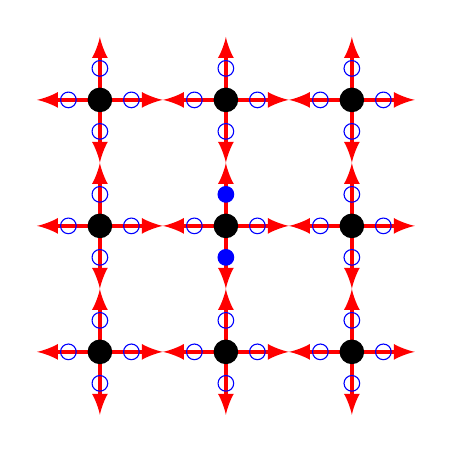
\begin{tikzpicture}[scale=0.4]
\foreach \x in {-4, 0, 4}
	{
	\foreach \y in {-4, 0, 4}
		{
		\ifthenelse{\x = 0 \AND \y = 0}{
    		\coordinate (Origin) at (0 + \x, 0 + \y);
    		\coordinate (site1) at (0+ \x,2+ \y);
    		\coordinate (site2) at (2+ \x,0+ \y);
    		\coordinate (site3) at (0+ \x,-2+ \y);
    		\coordinate (site4) at (-2+ \x,0+ \y);  
        
		\draw [ultra thick,-latex,red] (Origin)
   		     -- (site1) node [right] {};
    		\draw [ultra thick,-latex,red] (Origin)
        		-- (site2) node [below] {};
    		\draw [ultra thick,-latex,red] (Origin)
        		-- (site3) node [left] {};
    		\draw [ultra thick,-latex,red] (Origin)
        		-- (site4) node [above] {};
       
    		\node[draw,circle,inner sep=3pt,fill] at (0+ \x,0+ \y) {};
    		\node[draw,circle,inner sep=2pt,blue] at (1+ \x,0+ \y) {};
		\node[draw,circle,inner sep=2pt,fill,blue] at (0+ \x,1+ \y) {};
		\node[draw,circle,inner sep=2pt,blue] at (-1+ \x,0+ \y) {};
		\node[draw,circle,inner sep=2pt,fill,blue] at (0+ \x,-1+ \y) {};
		}%else
		{
		
    		\coordinate (Origin) at (0 + \x, 0 + \y);
    		\coordinate (site1) at (0+ \x,2+ \y);
    		\coordinate (site2) at (2+ \x,0+ \y);
    		\coordinate (site3) at (0+ \x,-2+ \y);
    		\coordinate (site4) at (-2+ \x,0+ \y);  
        
		\draw [ultra thick,-latex,red] (Origin)
   		     -- (site1) node [right] {};
    		\draw [ultra thick,-latex,red] (Origin)
        		-- (site2) node [below] {};
    		\draw [ultra thick,-latex,red] (Origin)
        		-- (site3) node [left] {};
    		\draw [ultra thick,-latex,red] (Origin)
        		-- (site4) node [above] {};
       
    		\node[draw,circle,inner sep=3pt,fill] at (0+ \x,0+ \y) {};
    		\node[draw,circle,inner sep=2pt,blue] at (1+ \x,0+ \y) {};
		\node[draw,circle,inner sep=2pt,blue] at (0+ \x,1+ \y) {};
		\node[draw,circle,inner sep=2pt,blue] at (-1+ \x,0+ \y) {};
		\node[draw,circle,inner sep=2pt,blue] at (0+ \x,-1+ \y) {};
		}
		}
	}
  \end{tikzpicture}
  \caption{After Collision and before propagation}
  \label{figure:propagation_HPP1} 
   \end{block}
   \end{minipage}
  \begin{minipage}{0.47\textwidth}
	\begin{block}{After}
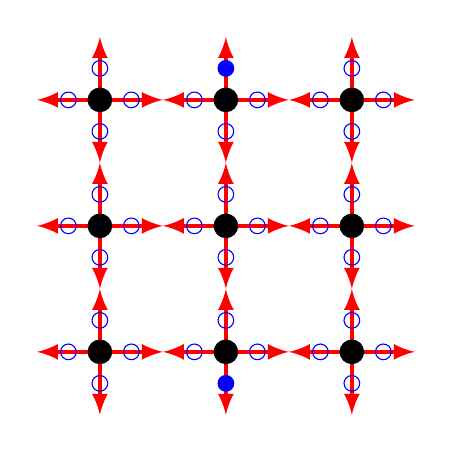
\begin{tikzpicture}[scale=0.4]
\foreach \x in {-4, 0, 4}
	{
	\foreach \y in {-4, 0, 4}
		{
		\ifthenelse{\x = 0 \AND \y = -4}{
    			\coordinate (Origin) at (0 + \x, 0 + \y);
    			\coordinate (site1) at (0+ \x,2+ \y);
    			\coordinate (site2) at (2+ \x,0+ \y);
    			\coordinate (site3) at (0+ \x,-2+ \y);
    			\coordinate (site4) at (-2+ \x,0+ \y);  
        
			\draw [ultra thick,-latex,red] (Origin)
   			     -- (site1) node [right] {};
    			\draw [ultra thick,-latex,red] (Origin)
        			-- (site2) node [below] {};
    			\draw [ultra thick,-latex,red] (Origin)
        			-- (site3) node [left] {};
    			\draw [ultra thick,-latex,red] (Origin)
        			-- (site4) node [above] {};
       
    			\node[draw,circle,inner sep=3pt,fill] at (0+ \x,0+ \y) {};
    			\node[draw,circle,inner sep=2pt,blue] at (1+ \x,0+ \y) {};
			\node[draw,circle,inner sep=2pt,blue] at (0+ \x,1+ \y) {};
			\node[draw,circle,inner sep=2pt,blue] at (-1+ \x,0+ \y) {};
			\node[draw,circle,inner sep=2pt,fill,blue] at (0+ \x,-1+ \y) {};
		}%else
		{
			\ifthenelse{\x = 0 \AND \y = 4}
				{
    					\coordinate (Origin) at (0 + \x, 0 + \y);
    					\coordinate (site1) at (0+ \x,2+ \y);
    					\coordinate (site2) at (2+ \x,0+ \y);
    					\coordinate (site3) at (0+ \x,-2+ \y);
    					\coordinate (site4) at (-2+ \x,0+ \y);  
        
					\draw [ultra thick,-latex,red] (Origin)
   					     -- (site1) node [right] {};
    					\draw [ultra thick,-latex,red] (Origin)
       	 				-- (site2) node [below] {};
    					\draw [ultra thick,-latex,red] (Origin)
       	 				-- (site3) node [left] {};
    					\draw [ultra thick,-latex,red] (Origin)
        					-- (site4) node [above] {};
       
    					\node[draw,circle,inner sep=3pt,fill] at (0+ \x,0+ \y) {};
    					\node[draw,circle,inner sep=2pt,blue] at (1+ \x,0+ \y) {};
					\node[draw,circle,inner sep=2pt,fill,blue] at (0+ \x,1+ \y) {};
					\node[draw,circle,inner sep=2pt,blue] at (-1+ \x,0+ \y) {};
					\node[draw,circle,inner sep=2pt,blue] at (0+ \x,-1+ \y) {};
				}% else
				{
					\coordinate (Origin) at (0 + \x, 0 + \y);
    					\coordinate (site1) at (0+ \x,2+ \y);
    					\coordinate (site2) at (2+ \x,0+ \y);
    					\coordinate (site3) at (0+ \x,-2+ \y);
    					\coordinate (site4) at (-2+ \x,0+ \y);  
        
					\draw [ultra thick,-latex,red] (Origin)
   					     -- (site1) node [right] {};
    					\draw [ultra thick,-latex,red] (Origin)
       	 				-- (site2) node [below] {};
    					\draw [ultra thick,-latex,red] (Origin)
       	 				-- (site3) node [left] {};
    					\draw [ultra thick,-latex,red] (Origin)
        					-- (site4) node [above] {};
       
    					\node[draw,circle,inner sep=3pt,fill] at (0+ \x,0+ \y) {};
    					\node[draw,circle,inner sep=2pt,blue] at (1+ \x,0+ \y) {};
					\node[draw,circle,inner sep=2pt,blue] at (0+ \x,1+ \y) {};
					\node[draw,circle,inner sep=2pt,blue] at (-1+ \x,0+ \y) {};
					\node[draw,circle,inner sep=2pt,blue] at (0+ \x,-1+ \y) {};
				}
			}
		}
	}
  \end{tikzpicture}
  \caption{After propagation}
  \label{figure:propagation_HPP1} 
   \end{block}
   \end{minipage}
	\end{frame}
	
	%six
	\subsection{HPP Mass and Momentum densities}
	\begin{frame}
	\frametitle{HPP Mass and Momentum densities}
	The \acrshort{lgca} can be fully describe by the boolean fields $n_{i}(t, \textbf{r}_{j})$, where $i \in \{0, 1, 2, 3\}$, \textbf{r} is the position of the cell and t is the discrete time. $n_{i}(t, \textbf{r}_{j})$ means the boolean value of the ith site at position \textbf{r} at time t.
Before calculating the mass and momentum densities we require the mean occupation numbers. The mean occupation number for site $i$ at position \textbf{x}, is the average of $n_{i}(t, \textbf{r}_{j})$ where 
$\textbf{r}_{j}$ are the the positions of the neighbours of \textbf{x}
\[N_{i}(t,\textbf{x}) = \frac{\sum_{j = 0}^{3} n_{i}(t,\textbf{r}_{j})}{4}.\]
The mass density for time t and position \textbf{x} is defined as follow:
\[\rho(t, \textbf{x}) = \sum_{i = 0}^{3} N_{i}(t, \textbf{x}).\]

	\end{frame}
	
	\subsection{HPP Mass and Momentum densities continued}
	\begin{frame}
	\frametitle{HPP Mass and Momentum densities continued}
	
    The momentum densities for time t and position \textbf{x} is defined as follow:
\[\boldsymbol{j}(t, \textbf{x}) = \rho\boldsymbol{u} = \sum_{i = 0}^{3} \textbf{c}_{i}N_{i}(t, \textbf{x}).\]
Given $\rho$ and $\boldsymbol{j}$ the mass and momentum densities we can calculate $N_{i}$ assuming
a linear relationship
\[N_{i} = \xi\rho + \eta\textbf{c}_{i}\boldsymbol{j}.\]
We get: $\xi = \frac{1}{4};$ and $\eta = \frac{1}{2}$ thus
	\[N_{i} =\frac{1}{4}\rho + \frac{1}{2}\textbf{c}_{i}\boldsymbol{j}.\]
	\end{frame}
	
	\section{FHP}
	\begin{frame}
	\frametitle{FHP}
	\minipage{0.45\textwidth}
    \begin{block}{History}
	\begin{itemize}
    \item Developed in 1986.
    \item By Frisch, Hasslacher and Pomeau.
    \item Navier-Stokes success.
    \item pauli exclusion principle.
    \item FHP-I, FHP-II and FHP-III.
    \end{itemize}
    \end{block}
    \endminipage\hfill
    \minipage{0.45\textwidth}
    \begin{block}{History}
    \begin{figure}[H]
  \centering
  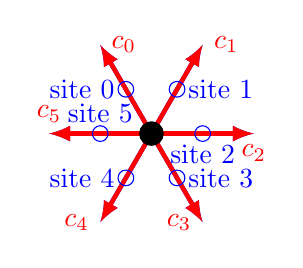
\begin{tikzpicture}[scale=0.65]
  \foreach \x in {0}
	{
	\foreach \y in {0}
		{
    \coordinate (Origin) at (0 + \x,0 + \y);
    \coordinate (site1) at ({2 * cos(120) + \x }, {2 * sin(120) + \y });
    \coordinate (site2) at ({2 * cos(60) + \x }, {2 * sin(60) + \y });
    \coordinate (site3) at ({2 * cos(0) + \x }, {2 * sin(0) + \y });
    \coordinate (site4) at ({2 * cos(-60) + \x }, {2 * sin(-60) + \y });
    \coordinate (site5) at ({2 * cos(-120) + \x }, {2 * sin(-120) + \y });
    \coordinate (site6) at ({2 * cos(-180) + \x }, {2 * sin(-180) + \y });
    
    \draw [ultra thick,-latex,blue] (Origin)
        -- (site1) node [midway, left] {site 0};
    \draw [ultra thick,-latex,blue] (Origin)
        -- (site2) node [midway, right] {site 1};
    \draw [ultra thick,-latex,blue] (Origin)
        -- (site3) node [midway, below] {site 2};
    \draw [ultra thick,-latex,blue] (Origin)
        -- (site4) node [midway, right] {site 3};
    \draw [ultra thick,-latex,blue] (Origin)
        -- (site5) node [midway, left] {site 4};
    \draw [ultra thick,-latex,blue] (Origin)
        -- (site6) node [midway, above] {site 5};     
	\draw [ultra thick,-latex,red] (Origin)
        -- (site1) node [right] {$c_0$};
    \draw [ultra thick,-latex,red] (Origin)
        -- (site2) node [right] {$c_1$};
    \draw [ultra thick,-latex,red] (Origin)
        -- (site3) node [below] {$c_2$};
    \draw [ultra thick,-latex,red] (Origin)
        -- (site4) node [left] {$c_3$};
    \draw [ultra thick,-latex,red] (Origin)
        -- (site5) node [left] {$c_4$};
    \draw [ultra thick,-latex,red] (Origin)
        -- (site6) node [above] {$c_5$};    
 \coordinate (Origin) at (0 + \x,0 + \y);
    \coordinate (site1) at ({cos(120) + \x }, { sin(120) + \y });
    \coordinate (site2) at ({ cos(60) + \x }, { sin(60) + \y });
    \coordinate (site3) at ({ cos(0) + \x }, { sin(0) + \y });
    \coordinate (site4) at ({ cos(-60) + \x }, { sin(-60) + \y });
    \coordinate (site5) at ({ cos(-120) + \x }, { sin(-120) + \y });
    \coordinate (site6) at ({ cos(-180) + \x }, { sin(-180) + \y });
       
    \node[draw,circle,inner sep=3pt,fill] at (Origin) {};
    \node[draw,circle,inner sep=2pt,blue] at (site1) {};
    \node[draw,circle,inner sep=2pt,blue] at (site2) {};
    \node[draw,circle,inner sep=2pt,blue] at (site3) {};
    \node[draw,circle,inner sep=2pt,blue] at (site4) {};
    \node[draw,circle,inner sep=2pt,blue] at (site5) {};
    \node[draw,circle,inner sep=2pt,blue] at (site6) {};
    }
 }
  \end{tikzpicture}
  \caption{Here is an example of a single hexagonal cell with 6 velocity vectors and 6 empty sites.}
  \label{figure:Hsingle-cell}
\end{figure}
\end{block}
    \endminipage\hfill
	\end{frame}
	
	%five
	\subsection{FHP Collision Phase1}
	\begin{frame}
	\frametitle{FHP Collision Phase1}
	\minipage{0.45\textwidth}
    \begin{block}{Before collision.}
      \begin{tikzpicture}[scale=0.4]
    \coordinate (Origin) at (0 + \x,0 + \y);
    \coordinate (site1) at ({2 * cos(120) + \x }, {2 * sin(120) + \y });
    \coordinate (site2) at ({2 * cos(60) + \x }, {2 * sin(60) + \y });
    \coordinate (site3) at ({2 * cos(0) + \x }, {2 * sin(0) + \y });
    \coordinate (site4) at ({2 * cos(-60) + \x }, {2 * sin(-60) + \y });
    \coordinate (site5) at ({2 * cos(-120) + \x }, {2 * sin(-120) + \y });
    \coordinate (site6) at ({2 * cos(-180) + \x }, {2 * sin(-180) + \y });
    
	\draw [ultra thick,-latex,red] (Origin)
        -- (site1) node [right] {};
    \draw [ultra thick,-latex,red] (Origin)
        -- (site2) node [right] {};
    \draw [ultra thick,-latex,red] (Origin)
        -- (site3) node [below] {};
    \draw [ultra thick,-latex,red] (Origin)
        -- (site4) node [left] {};
    \draw [ultra thick,-latex,red] (Origin)
        -- (site5) node [left] {};
    \draw [ultra thick,-latex,red] (Origin)
        -- (site6) node [above] {};    
 \coordinate (Origin) at (0 + \x,0 + \y);
    \coordinate (site1) at ({cos(120) + \x }, { sin(120) + \y });
    \coordinate (site2) at ({ cos(60) + \x }, { sin(60) + \y });
    \coordinate (site3) at ({ cos(0) + \x }, { sin(0) + \y });
    \coordinate (site4) at ({ cos(-60) + \x }, { sin(-60) + \y });
    \coordinate (site5) at ({ cos(-120) + \x }, { sin(-120) + \y });
    \coordinate (site6) at ({ cos(-180) + \x }, { sin(-180) + \y });
       
    \node[draw,circle,inner sep=3pt,fill] at (Origin) {};
    \node[draw,circle,inner sep=2pt,fill,blue] at (site1) {};
    \node[draw,circle,inner sep=2pt,blue] at (site2) {};
    \node[draw,circle,inner sep=2pt,blue] at (site3) {};
    \node[draw,circle,inner sep=2pt,fill,blue] at (site4) {};
    \node[draw,circle,inner sep=2pt,blue] at (site5) {};
    \node[draw,circle,inner sep=2pt,blue] at (site6) {};
  \end{tikzpicture}
  \caption{Before collision.}
    \end{block}
    \endminipage\hfill
    \minipage{0.45\textwidth}
    \begin{block}{First possible outcome.}
    \begin{tikzpicture}[scale=0.4]
    \coordinate (Origin) at (0 + \x,0 + \y);
    \coordinate (site1) at ({2 * cos(120) + \x }, {2 * sin(120) + \y });
    \coordinate (site2) at ({2 * cos(60) + \x }, {2 * sin(60) + \y });
    \coordinate (site3) at ({2 * cos(0) + \x }, {2 * sin(0) + \y });
    \coordinate (site4) at ({2 * cos(-60) + \x }, {2 * sin(-60) + \y });
    \coordinate (site5) at ({2 * cos(-120) + \x }, {2 * sin(-120) + \y });
    \coordinate (site6) at ({2 * cos(-180) + \x }, {2 * sin(-180) + \y });    
	\draw [ultra thick,-latex,red] (Origin)
        -- (site1) node [right] {};
    \draw [ultra thick,-latex,red] (Origin)
        -- (site2) node [right] {};
    \draw [ultra thick,-latex,red] (Origin)
        -- (site3) node [below] {};
    \draw [ultra thick,-latex,red] (Origin)
        -- (site4) node [left] {};
    \draw [ultra thick,-latex,red] (Origin)
        -- (site5) node [left] {};
    \draw [ultra thick,-latex,red] (Origin)
        -- (site6) node [above] {};    
    \coordinate (Origin) at (0 + \x,0 + \y);
    \coordinate (site1) at ({cos(120) + \x }, { sin(120) + \y });
    \coordinate (site2) at ({ cos(60) + \x }, { sin(60) + \y });
    \coordinate (site3) at ({ cos(0) + \x }, { sin(0) + \y });
    \coordinate (site4) at ({ cos(-60) + \x }, { sin(-60) + \y });
    \coordinate (site5) at ({ cos(-120) + \x }, { sin(-120) + \y });
    \coordinate (site6) at ({ cos(-180) + \x }, { sin(-180) + \y });
       
    \node[draw,circle,inner sep=3pt,fill] at (Origin) {};
    \node[draw,circle,inner sep=2pt,blue] at (site1) {};
    \node[draw,circle,inner sep=2pt,blue] at (site2) {};
    \node[draw,circle,inner sep=2pt,fill,blue] at (site3) {};
    \node[draw,circle,inner sep=2pt,blue] at (site4) {};
    \node[draw,circle,inner sep=2pt,blue] at (site5) {};
    \node[draw,circle,inner sep=2pt,fill,blue] at (site6) {};
  \end{tikzpicture}
  \caption{First possible outcome.}
    \end{block}
    \endminipage\hfill
     
     \minipage{0.45\textwidth}
    \begin{block}{Second possible outcome.}
    \begin{tikzpicture}[scale=0.4]
    \coordinate (Origin) at (0 + \x,0 + \y);
    \coordinate (site1) at ({2 * cos(120) + \x }, {2 * sin(120) + \y });
    \coordinate (site2) at ({2 * cos(60) + \x }, {2 * sin(60) + \y });
    \coordinate (site3) at ({2 * cos(0) + \x }, {2 * sin(0) + \y });
    \coordinate (site4) at ({2 * cos(-60) + \x }, {2 * sin(-60) + \y });
    \coordinate (site5) at ({2 * cos(-120) + \x }, {2 * sin(-120) + \y });
    \coordinate (site6) at ({2 * cos(-180) + \x }, {2 * sin(-180) + \y });    
	\draw [ultra thick,-latex,red] (Origin)
        -- (site1) node [right] {};
    \draw [ultra thick,-latex,red] (Origin)
        -- (site2) node [right] {};
    \draw [ultra thick,-latex,red] (Origin)
        -- (site3) node [below] {};
    \draw [ultra thick,-latex,red] (Origin)
        -- (site4) node [left] {};
    \draw [ultra thick,-latex,red] (Origin)
        -- (site5) node [left] {};
    \draw [ultra thick,-latex,red] (Origin)
        -- (site6) node [above] {};    
    \coordinate (Origin) at (0 + \x,0 + \y);
    \coordinate (site1) at ({cos(120) + \x }, { sin(120) + \y });
    \coordinate (site2) at ({ cos(60) + \x }, { sin(60) + \y });
    \coordinate (site3) at ({ cos(0) + \x }, { sin(0) + \y });
    \coordinate (site4) at ({ cos(-60) + \x }, { sin(-60) + \y });
    \coordinate (site5) at ({ cos(-120) + \x }, { sin(-120) + \y });
    \coordinate (site6) at ({ cos(-180) + \x }, { sin(-180) + \y });
       
    \node[draw,circle,inner sep=3pt,fill] at (Origin) {};
    \node[draw,circle,inner sep=2pt,blue] at (site1) {};
    \node[draw,circle,inner sep=2pt,fill,blue] at (site2) {};
    \node[draw,circle,inner sep=2pt,blue] at (site3) {};
    \node[draw,circle,inner sep=2pt,blue] at (site4) {};
    \node[draw,circle,inner sep=2pt,fill,blue] at (site5) {};
    \node[draw,circle,inner sep=2pt,blue] at (site6) {};
  \end{tikzpicture}
  \caption{Second possible outcome.}
        \end{block}
    \endminipage\hfill

	\end{frame}
	
	\subsection{FHP Collision Phase2}
	\begin{frame}
	\frametitle{FHP Collision Phase2}
	\minipage{0.45\textwidth}
    \begin{block}{Before collision.}
    \begin{tikzpicture}[scale=0.4]
    \coordinate (Origin) at (0 + \x,0 + \y);
    \coordinate (site1) at ({2 * cos(120) + \x }, {2 * sin(120) + \y });
    \coordinate (site2) at ({2 * cos(60) + \x }, {2 * sin(60) + \y });
    \coordinate (site3) at ({2 * cos(0) + \x }, {2 * sin(0) + \y });
    \coordinate (site4) at ({2 * cos(-60) + \x }, {2 * sin(-60) + \y });
    \coordinate (site5) at ({2 * cos(-120) + \x }, {2 * sin(-120) + \y });
    \coordinate (site6) at ({2 * cos(-180) + \x }, {2 * sin(-180) + \y });
    
	\draw [ultra thick,-latex,red] (Origin)
        -- (site1) node [right] {};
    \draw [ultra thick,-latex,red] (Origin)
        -- (site2) node [right] {};
    \draw [ultra thick,-latex,red] (Origin)
        -- (site3) node [below] {};
    \draw [ultra thick,-latex,red] (Origin)
        -- (site4) node [left] {};
    \draw [ultra thick,-latex,red] (Origin)
        -- (site5) node [left] {};
    \draw [ultra thick,-latex,red] (Origin)
        -- (site6) node [above] {};    
 \coordinate (Origin) at (0 + \x,0 + \y);
    \coordinate (site1) at ({cos(120) + \x }, { sin(120) + \y });
    \coordinate (site2) at ({ cos(60) + \x }, { sin(60) + \y });
    \coordinate (site3) at ({ cos(0) + \x }, { sin(0) + \y });
    \coordinate (site4) at ({ cos(-60) + \x }, { sin(-60) + \y });
    \coordinate (site5) at ({ cos(-120) + \x }, { sin(-120) + \y });
    \coordinate (site6) at ({ cos(-180) + \x }, { sin(-180) + \y });
       
    \node[draw,circle,inner sep=3pt,fill] at (Origin) {};
    \node[draw,circle,inner sep=2pt,blue] at (site1) {};
    \node[draw,circle,inner sep=2pt,fill,blue] at (site2) {};
    \node[draw,circle,inner sep=2pt,blue] at (site3) {};
    \node[draw,circle,inner sep=2pt,fill,blue] at (site4) {};
    \node[draw,circle,inner sep=2pt,blue] at (site5) {};
    \node[draw,circle,inner sep=2pt,fill,blue] at (site6) {};
  \end{tikzpicture}
  \caption{Before collision.}
        \end{block}
    \endminipage\hfill
    \minipage{0.45\textwidth}
    \begin{block}{After collision.}
    \begin{tikzpicture}[scale=0.4]
    \coordinate (Origin) at (0 + \x,0 + \y);
    \coordinate (site1) at ({2 * cos(120) + \x }, {2 * sin(120) + \y });
    \coordinate (site2) at ({2 * cos(60) + \x }, {2 * sin(60) + \y });
    \coordinate (site3) at ({2 * cos(0) + \x }, {2 * sin(0) + \y });
    \coordinate (site4) at ({2 * cos(-60) + \x }, {2 * sin(-60) + \y });
    \coordinate (site5) at ({2 * cos(-120) + \x }, {2 * sin(-120) + \y });
    \coordinate (site6) at ({2 * cos(-180) + \x }, {2 * sin(-180) + \y });    
	\draw [ultra thick,-latex,red] (Origin)
        -- (site1) node [right] {};
    \draw [ultra thick,-latex,red] (Origin)
        -- (site2) node [right] {};
    \draw [ultra thick,-latex,red] (Origin)
        -- (site3) node [below] {};
    \draw [ultra thick,-latex,red] (Origin)
        -- (site4) node [left] {};
    \draw [ultra thick,-latex,red] (Origin)
        -- (site5) node [left] {};
    \draw [ultra thick,-latex,red] (Origin)
        -- (site6) node [above] {};    
    \coordinate (Origin) at (0 + \x,0 + \y);
    \coordinate (site1) at ({cos(120) + \x }, { sin(120) + \y });
    \coordinate (site2) at ({ cos(60) + \x }, { sin(60) + \y });
    \coordinate (site3) at ({ cos(0) + \x }, { sin(0) + \y });
    \coordinate (site4) at ({ cos(-60) + \x }, { sin(-60) + \y });
    \coordinate (site5) at ({ cos(-120) + \x }, { sin(-120) + \y });
    \coordinate (site6) at ({ cos(-180) + \x }, { sin(-180) + \y });
       
    \node[draw,circle,inner sep=3pt,fill] at (Origin) {};
    \node[draw,circle,inner sep=2pt,fill,blue] at (site1) {};
    \node[draw,circle,inner sep=2pt,blue] at (site2) {};
    \node[draw,circle,inner sep=2pt,fill,blue] at (site3) {};
    \node[draw,circle,inner sep=2pt,blue] at (site4) {};
    \node[draw,circle,inner sep=2pt,fill,blue] at (site5) {};
    \node[draw,circle,inner sep=2pt,blue] at (site6) {};
  \end{tikzpicture}
  \caption{After collision.}	
	    \end{block}
    \endminipage\hfill
	\end{frame}
	
	\subsection{FHP Collision Phase3}
	\begin{frame}
	\frametitle{FHP Collision Phase3}
	\minipage{0.45\textwidth}
    \begin{block}{Before collision.}
    \begin{tikzpicture}[scale=0.4]
    \coordinate (Origin) at (0 + \x,0 + \y);
    \coordinate (site1) at ({2 * cos(120) + \x }, {2 * sin(120) + \y });
    \coordinate (site2) at ({2 * cos(60) + \x }, {2 * sin(60) + \y });
    \coordinate (site3) at ({2 * cos(0) + \x }, {2 * sin(0) + \y });
    \coordinate (site4) at ({2 * cos(-60) + \x }, {2 * sin(-60) + \y });
    \coordinate (site5) at ({2 * cos(-120) + \x }, {2 * sin(-120) + \y });
    \coordinate (site6) at ({2 * cos(-180) + \x }, {2 * sin(-180) + \y });
    
	\draw [ultra thick,-latex,red] (Origin)
        -- (site1) node [right] {};
    \draw [ultra thick,-latex,red] (Origin)
        -- (site2) node [right] {};
    \draw [ultra thick,-latex,red] (Origin)
        -- (site3) node [below] {};
    \draw [ultra thick,-latex,red] (Origin)
        -- (site4) node [left] {};
    \draw [ultra thick,-latex,red] (Origin)
        -- (site5) node [left] {};
    \draw [ultra thick,-latex,red] (Origin)
        -- (site6) node [above] {};    
 \coordinate (Origin) at (0 + \x,0 + \y);
    \coordinate (site1) at ({cos(120) + \x }, { sin(120) + \y });
    \coordinate (site2) at ({ cos(60) + \x }, { sin(60) + \y });
    \coordinate (site3) at ({ cos(0) + \x }, { sin(0) + \y });
    \coordinate (site4) at ({ cos(-60) + \x }, { sin(-60) + \y });
    \coordinate (site5) at ({ cos(-120) + \x }, { sin(-120) + \y });
    \coordinate (site6) at ({ cos(-180) + \x }, { sin(-180) + \y });
       
    \node[draw,circle,inner sep=3pt,fill] at (Origin) {};
    \node[draw,circle,inner sep=2pt,fill,blue] at (site1) {};
    \node[draw,circle,inner sep=2pt,fill,blue] at (site2) {};
    \node[draw,circle,inner sep=2pt,blue] at (site3) {};
    \node[draw,circle,inner sep=2pt,fill,blue] at (site4) {};
    \node[draw,circle,inner sep=2pt,fill,blue] at (site5) {};
    \node[draw,circle,inner sep=2pt,blue] at (site6) {};
  \end{tikzpicture}
  \caption{Before collision.}
        \end{block}
    \endminipage\hfill
    \minipage{0.45\textwidth}
    \begin{block}{First possible outcome.}
    \begin{tikzpicture}[scale=0.4]
    \coordinate (Origin) at (0 + \x,0 + \y);
    \coordinate (site1) at ({2 * cos(120) + \x }, {2 * sin(120) + \y });
    \coordinate (site2) at ({2 * cos(60) + \x }, {2 * sin(60) + \y });
    \coordinate (site3) at ({2 * cos(0) + \x }, {2 * sin(0) + \y });
    \coordinate (site4) at ({2 * cos(-60) + \x }, {2 * sin(-60) + \y });
    \coordinate (site5) at ({2 * cos(-120) + \x }, {2 * sin(-120) + \y });
    \coordinate (site6) at ({2 * cos(-180) + \x }, {2 * sin(-180) + \y });    
	\draw [ultra thick,-latex,red] (Origin)
        -- (site1) node [right] {};
    \draw [ultra thick,-latex,red] (Origin)
        -- (site2) node [right] {};
    \draw [ultra thick,-latex,red] (Origin)
        -- (site3) node [below] {};
    \draw [ultra thick,-latex,red] (Origin)
        -- (site4) node [left] {};
    \draw [ultra thick,-latex,red] (Origin)
        -- (site5) node [left] {};
    \draw [ultra thick,-latex,red] (Origin)
        -- (site6) node [above] {};    
    \coordinate (Origin) at (0 + \x,0 + \y);
    \coordinate (site1) at ({cos(120) + \x }, { sin(120) + \y });
    \coordinate (site2) at ({ cos(60) + \x }, { sin(60) + \y });
    \coordinate (site3) at ({ cos(0) + \x }, { sin(0) + \y });
    \coordinate (site4) at ({ cos(-60) + \x }, { sin(-60) + \y });
    \coordinate (site5) at ({ cos(-120) + \x }, { sin(-120) + \y });
    \coordinate (site6) at ({ cos(-180) + \x }, { sin(-180) + \y });
       
    \node[draw,circle,inner sep=3pt,fill] at (Origin) {};
    \node[draw,circle,inner sep=2pt,fill,blue] at (site1) {};
    \node[draw,circle,inner sep=2pt,blue] at (site2) {};
    \node[draw,circle,inner sep=2pt,fill,blue] at (site3) {};
    \node[draw,circle,inner sep=2pt,fill,blue] at (site4) {};
    \node[draw,circle,inner sep=2pt,blue] at (site5) {};
    \node[draw,circle,inner sep=2pt,fill,blue] at (site6) {};
  \end{tikzpicture}
  \caption{First possible outcome.}
    \end{block}
    \endminipage\hfill
        \minipage{0.45\textwidth}
    \begin{block}{Second possible outcome.}
    \begin{tikzpicture}[scale=0.4]
    \coordinate (Origin) at (0 + \x,0 + \y);
    \coordinate (site1) at ({2 * cos(120) + \x }, {2 * sin(120) + \y });
    \coordinate (site2) at ({2 * cos(60) + \x }, {2 * sin(60) + \y });
    \coordinate (site3) at ({2 * cos(0) + \x }, {2 * sin(0) + \y });
    \coordinate (site4) at ({2 * cos(-60) + \x }, {2 * sin(-60) + \y });
    \coordinate (site5) at ({2 * cos(-120) + \x }, {2 * sin(-120) + \y });
    \coordinate (site6) at ({2 * cos(-180) + \x }, {2 * sin(-180) + \y });    
	\draw [ultra thick,-latex,red] (Origin)
        -- (site1) node [right] {};
    \draw [ultra thick,-latex,red] (Origin)
        -- (site2) node [right] {};
    \draw [ultra thick,-latex,red] (Origin)
        -- (site3) node [below] {};
    \draw [ultra thick,-latex,red] (Origin)
        -- (site4) node [left] {};
    \draw [ultra thick,-latex,red] (Origin)
        -- (site5) node [left] {};
    \draw [ultra thick,-latex,red] (Origin)
        -- (site6) node [above] {};    
    \coordinate (Origin) at (0 + \x,0 + \y);
    \coordinate (site1) at ({cos(120) + \x }, { sin(120) + \y });
    \coordinate (site2) at ({ cos(60) + \x }, { sin(60) + \y });
    \coordinate (site3) at ({ cos(0) + \x }, { sin(0) + \y });
    \coordinate (site4) at ({ cos(-60) + \x }, { sin(-60) + \y });
    \coordinate (site5) at ({ cos(-120) + \x }, { sin(-120) + \y });
    \coordinate (site6) at ({ cos(-180) + \x }, { sin(-180) + \y });
       
    \node[draw,circle,inner sep=3pt,fill] at (Origin) {};
    \node[draw,circle,inner sep=2pt,blue] at (site1) {};
    \node[draw,circle,inner sep=2pt,fill,blue] at (site2) {};
    \node[draw,circle,inner sep=2pt,fill,blue] at (site3) {};
    \node[draw,circle,inner sep=2pt,blue] at (site4) {};
    \node[draw,circle,inner sep=2pt,fill,blue] at (site5) {};
    \node[draw,circle,inner sep=2pt,fill,blue] at (site6) {};
  \end{tikzpicture}
  \caption{Second possible outcome.}
        \end{block}
    \endminipage\hfill
	\end{frame}
	
	\subsection{FHP Collision Phase4}
	\begin{frame}
	\frametitle{FHP Collision Phase4}
	\minipage{0.45\textwidth}
    \begin{block}{Before collision.}

  \begin{tikzpicture}[scale=0.4]
    \coordinate (Origin) at (0 + \x,0 + \y);
    \coordinate (site1) at ({2 * cos(120) + \x }, {2 * sin(120) + \y });
    \coordinate (site2) at ({2 * cos(60) + \x }, {2 * sin(60) + \y });
    \coordinate (site3) at ({2 * cos(0) + \x }, {2 * sin(0) + \y });
    \coordinate (site4) at ({2 * cos(-60) + \x }, {2 * sin(-60) + \y });
    \coordinate (site5) at ({2 * cos(-120) + \x }, {2 * sin(-120) + \y });
    \coordinate (site6) at ({2 * cos(-180) + \x }, {2 * sin(-180) + \y });
    
	\draw [ultra thick,-latex,red] (Origin)
        -- (site1) node [right] {};
    \draw [ultra thick,-latex,red] (Origin)
        -- (site2) node [right] {};
    \draw [ultra thick,-latex,red] (Origin)
        -- (site3) node [below] {};
    \draw [ultra thick,-latex,red] (Origin)
        -- (site4) node [left] {};
    \draw [ultra thick,-latex,red] (Origin)
        -- (site5) node [left] {};
    \draw [ultra thick,-latex,red] (Origin)
        -- (site6) node [above] {};    
 \coordinate (Origin) at (0 + \x,0 + \y);
    \coordinate (site1) at ({cos(120) + \x }, { sin(120) + \y });
    \coordinate (site2) at ({ cos(60) + \x }, { sin(60) + \y });
    \coordinate (site3) at ({ cos(0) + \x }, { sin(0) + \y });
    \coordinate (site4) at ({ cos(-60) + \x }, { sin(-60) + \y });
    \coordinate (site5) at ({ cos(-120) + \x }, { sin(-120) + \y });
    \coordinate (site6) at ({ cos(-180) + \x }, { sin(-180) + \y });
       
    \node[draw,circle,inner sep=3pt,fill] at (Origin) {};
    \node[draw,circle,inner sep=2pt,blue] at (site1) {};
    \node[draw,circle,inner sep=2pt,fill,blue] at (site2) {};
    \node[draw,circle,inner sep=2pt,blue] at (site3) {};
    \node[draw,circle,inner sep=2pt,blue] at (site4) {};
    \node[draw,circle,inner sep=2pt,fill,blue] at (site5) {};
    \node[draw,circle,inner sep=2pt,fill,blue] at (site6) {};
  \end{tikzpicture}
  \caption{Before collision.}
        \end{block}
    \endminipage\hfill
    \minipage{0.45\textwidth}
    \begin{block}{After collision.}
     \begin{tikzpicture}[scale=0.4]
    \coordinate (Origin) at (0 + \x,0 + \y);
    \coordinate (site1) at ({2 * cos(120) + \x }, {2 * sin(120) + \y });
    \coordinate (site2) at ({2 * cos(60) + \x }, {2 * sin(60) + \y });
    \coordinate (site3) at ({2 * cos(0) + \x }, {2 * sin(0) + \y });
    \coordinate (site4) at ({2 * cos(-60) + \x }, {2 * sin(-60) + \y });
    \coordinate (site5) at ({2 * cos(-120) + \x }, {2 * sin(-120) + \y });
    \coordinate (site6) at ({2 * cos(-180) + \x }, {2 * sin(-180) + \y });    
	\draw [ultra thick,-latex,red] (Origin)
        -- (site1) node [right] {};
    \draw [ultra thick,-latex,red] (Origin)
        -- (site2) node [right] {};
    \draw [ultra thick,-latex,red] (Origin)
        -- (site3) node [below] {};
    \draw [ultra thick,-latex,red] (Origin)
        -- (site4) node [left] {};
    \draw [ultra thick,-latex,red] (Origin)
        -- (site5) node [left] {};
    \draw [ultra thick,-latex,red] (Origin)
        -- (site6) node [above] {};    
    \coordinate (Origin) at (0 + \x,0 + \y);
    \coordinate (site1) at ({cos(120) + \x }, { sin(120) + \y });
    \coordinate (site2) at ({ cos(60) + \x }, { sin(60) + \y });
    \coordinate (site3) at ({ cos(0) + \x }, { sin(0) + \y });
    \coordinate (site4) at ({ cos(-60) + \x }, { sin(-60) + \y });
    \coordinate (site5) at ({ cos(-120) + \x }, { sin(-120) + \y });
    \coordinate (site6) at ({ cos(-180) + \x }, { sin(-180) + \y });
       
    \node[draw,circle,inner sep=3pt,fill] at (Origin) {};
    \node[draw,circle,inner sep=2pt,fill,blue] at (site1) {};
    \node[draw,circle,inner sep=2pt,blue] at (site2) {};
    \node[draw,circle,inner sep=2pt,blue] at (site3) {};
    \node[draw,circle,inner sep=2pt,fill,blue] at (site4) {};
    \node[draw,circle,inner sep=2pt,blue] at (site5) {};
    \node[draw,circle,inner sep=2pt,fill,blue] at (site6) {};
  \end{tikzpicture}
  \caption{After collision.}
        \end{block}
    \endminipage\hfill
	\end{frame}
	
	
	
	%six
	\subsection{FHP Propagation Phase}
	\begin{frame}
	\frametitle{FHP Propagation Phase}
	\centering
	\minipage{0.7\textwidth}
    \begin{block}{History}
      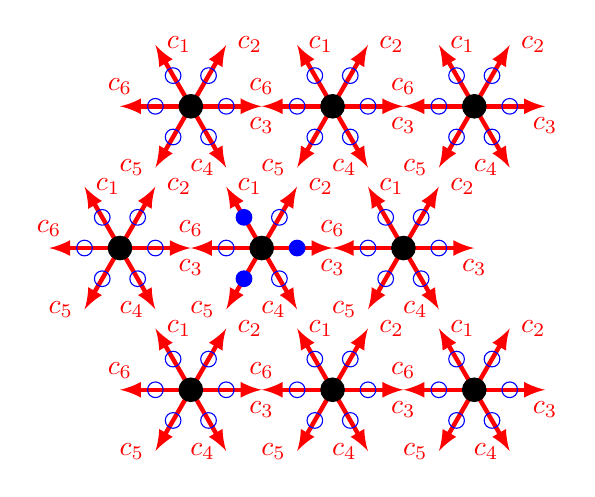
\begin{tikzpicture}[scale=0.45]
  \foreach \x in {0,4,8}
	{
	\foreach \y in {0,4,8}
		{
		\ifthenelse{\y = 4 }{
    			\coordinate (Origin) at (0 + \x - 2,0 + \y);
    			\coordinate (site1) at ({2 * cos(120) + \x- 2 }, {2 * sin(120) + \y });
    			\coordinate (site2) at ({2 * cos(60) + \x - 2}, {2 * sin(60) + \y });
    			\coordinate (site3) at ({2 * cos(0) + \x - 2}, {2 * sin(0) + \y });
    			\coordinate (site4) at ({2 * cos(-60) + \x - 2}, {2 * sin(-60) + \y });
    			\coordinate (site5) at ({2 * cos(-120) + \x - 2}, {2 * sin(-120) + \y });
    			\coordinate (site6) at ({2 * cos(-180) + \x- 2 }, {2 * sin(-180) + \y });
    
			\draw [ultra thick,-latex,red] (Origin)
        		-- (site1) node [right] {$c_1$};
    			\draw [ultra thick,-latex,red] (Origin)
        		-- (site2) node [right] {$c_2$};
    			\draw [ultra thick,-latex,red] (Origin)
        		-- (site3) node [below] {$c_3$};
    			\draw [ultra thick,-latex,red] (Origin)
        		-- (site4) node [left] {$c_4$};
    			\draw [ultra thick,-latex,red] (Origin)
        		-- (site5) node [left] {$c_5$};
    			\draw [ultra thick,-latex,red] (Origin)
        		-- (site6) node [above] {$c_6$};    
 			\coordinate (Origin) at (0 + \x- 2,0 + \y);
   			\coordinate (site1) at ({cos(120) + \x- 2 }, { sin(120) + \y });
   	 		\coordinate (site2) at ({ cos(60) + \x - 2}, { sin(60) + \y });
    			\coordinate (site3) at ({ cos(0) + \x- 2 }, { sin(0) + \y });
    			\coordinate (site4) at ({ cos(-60) + \x - 2}, { sin(-60) + \y });
    			\coordinate (site5) at ({ cos(-120) + \x - 2}, { sin(-120) + \y });
    			\coordinate (site6) at ({ cos(-180) + \x- 2 }, { sin(-180) + \y });
       
       		\ifthenelse{\x = 4 }{
    				\node[draw,circle,inner sep=3pt,fill] at (Origin) {};
    				\node[draw,circle,inner sep=2pt,fill,blue] at (site1) {};
    				\node[draw,circle,inner sep=2pt,blue] at (site2) {};
    				\node[draw,circle,inner sep=2pt,fill,blue] at (site3) {};
    				\node[draw,circle,inner sep=2pt,blue] at (site4) {};
    				\node[draw,circle,inner sep=2pt,fill,blue] at (site5) {};
    				\node[draw,circle,inner sep=2pt,blue] at (site6) {};
    			}%else
    			{
    				\node[draw,circle,inner sep=3pt,fill] at (Origin) {};
    				\node[draw,circle,inner sep=2pt,blue] at (site1) {};
    				\node[draw,circle,inner sep=2pt,blue] at (site2) {};
    				\node[draw,circle,inner sep=2pt,blue] at (site3) {};
    				\node[draw,circle,inner sep=2pt,blue] at (site4) {};
    				\node[draw,circle,inner sep=2pt,blue] at (site5) {};
    				\node[draw,circle,inner sep=2pt,blue] at (site6) {};
    			}
    }
    %else
    {
       	\coordinate (Origin) at (0 + \x ,0 + \y);
    		\coordinate (site1) at ({2 * cos(120) + \x }, {2 * sin(120) + \y });
    		\coordinate (site2) at ({2 * cos(60) + \x }, {2 * sin(60) + \y });
    		\coordinate (site3) at ({2 * cos(0) + \x }, {2 * sin(0) + \y });
    		\coordinate (site4) at ({2 * cos(-60) + \x }, {2 * sin(-60) + \y });
    		\coordinate (site5) at ({2 * cos(-120) + \x }, {2 * sin(-120) + \y });
    		\coordinate (site6) at ({2 * cos(-180) + \x}, {2 * sin(-180) + \y });    
		\draw [ultra thick,-latex,red] (Origin)
        -- (site1) node [right] {$c_1$};
    		\draw [ultra thick,-latex,red] (Origin)
        -- (site2) node [right] {$c_2$};
    		\draw [ultra thick,-latex,red] (Origin)
        -- (site3) node [below] {$c_3$};
    		\draw [ultra thick,-latex,red] (Origin)
        -- (site4) node [left] {$c_4$};
    		\draw [ultra thick,-latex,red] (Origin)
        -- (site5) node [left] {$c_5$};
    		\draw [ultra thick,-latex,red] (Origin)
        	-- (site6) node [above] {$c_6$};    
 		\coordinate (Origin) at (0 + \x,0 + \y);
    		\coordinate (site1) at ({cos(120) + \x }, { sin(120) + \y });
    		\coordinate (site2) at ({ cos(60) + \x }, { sin(60) + \y });
    		\coordinate (site3) at ({ cos(0) + \x}, { sin(0) + \y });
    		\coordinate (site4) at ({ cos(-60) + \x }, { sin(-60) + \y });
    		\coordinate (site5) at ({ cos(-120) + \x }, { sin(-120) + \y });
    		\coordinate (site6) at ({ cos(-180) + \x }, { sin(-180) + \y });
       
    		\node[draw,circle,inner sep=3pt,fill] at (Origin) {};
    		\node[draw,circle,inner sep=2pt,blue] at (site1) {};
    		\node[draw,circle,inner sep=2pt,blue] at (site2) {};
    		\node[draw,circle,inner sep=2pt,blue] at (site3) {};
    		\node[draw,circle,inner sep=2pt,blue] at (site4) {};
    		\node[draw,circle,inner sep=2pt,blue] at (site5) {};
    		\node[draw,circle,inner sep=2pt,blue] at (site6) {};
    }
    }
 }
  \end{tikzpicture}
  \caption{Before collision phase}
        \end{block}
    \endminipage\hfill
    
	\end{frame}
	
	\subsection{FHP Propagation Phase}
	\begin{frame}
	\frametitle{FHP Propagation Phase}
	\centering
	\minipage{0.7\textwidth}
    \begin{block}{After collision phase and before propagation phase.}
    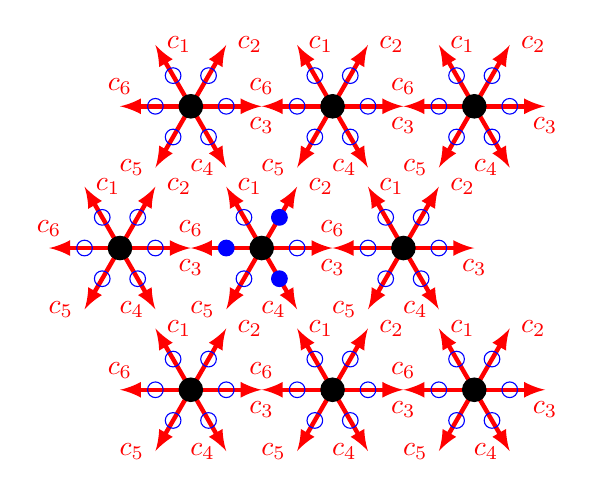
\begin{tikzpicture}[scale=0.45]
  \foreach \x in {0,4,8}
	{
	\foreach \y in {0,4,8}
		{
		\ifthenelse{\y = 4 }{
    			\coordinate (Origin) at (0 + \x - 2,0 + \y);
    			\coordinate (site1) at ({2 * cos(120) + \x- 2 }, {2 * sin(120) + \y });
    			\coordinate (site2) at ({2 * cos(60) + \x - 2}, {2 * sin(60) + \y });
    			\coordinate (site3) at ({2 * cos(0) + \x - 2}, {2 * sin(0) + \y });
    			\coordinate (site4) at ({2 * cos(-60) + \x - 2}, {2 * sin(-60) + \y });
    			\coordinate (site5) at ({2 * cos(-120) + \x - 2}, {2 * sin(-120) + \y });
    			\coordinate (site6) at ({2 * cos(-180) + \x- 2 }, {2 * sin(-180) + \y });
    
			\draw [ultra thick,-latex,red] (Origin)
        		-- (site1) node [right] {$c_1$};
    			\draw [ultra thick,-latex,red] (Origin)
        		-- (site2) node [right] {$c_2$};
    			\draw [ultra thick,-latex,red] (Origin)
        		-- (site3) node [below] {$c_3$};
    			\draw [ultra thick,-latex,red] (Origin)
        		-- (site4) node [left] {$c_4$};
    			\draw [ultra thick,-latex,red] (Origin)
        		-- (site5) node [left] {$c_5$};
    			\draw [ultra thick,-latex,red] (Origin)
        		-- (site6) node [above] {$c_6$};    
 			\coordinate (Origin) at (0 + \x- 2,0 + \y);
   			\coordinate (site1) at ({cos(120) + \x- 2 }, { sin(120) + \y });
   	 		\coordinate (site2) at ({ cos(60) + \x - 2}, { sin(60) + \y });
    			\coordinate (site3) at ({ cos(0) + \x- 2 }, { sin(0) + \y });
    			\coordinate (site4) at ({ cos(-60) + \x - 2}, { sin(-60) + \y });
    			\coordinate (site5) at ({ cos(-120) + \x - 2}, { sin(-120) + \y });
    			\coordinate (site6) at ({ cos(-180) + \x- 2 }, { sin(-180) + \y });
       
       		\ifthenelse{\x = 4 }{
    				\node[draw,circle,inner sep=3pt,fill] at (Origin) {};
    				\node[draw,circle,inner sep=2pt,blue] at (site1) {};
    				\node[draw,circle,inner sep=2pt,fill,blue] at (site2) {};
    				\node[draw,circle,inner sep=2pt,blue] at (site3) {};
    				\node[draw,circle,inner sep=2pt,fill,blue] at (site4) {};
    				\node[draw,circle,inner sep=2pt,blue] at (site5) {};
    				\node[draw,circle,inner sep=2pt,fill,blue] at (site6) {};
    			}%else
    			{
    				\node[draw,circle,inner sep=3pt,fill] at (Origin) {};
    				\node[draw,circle,inner sep=2pt,blue] at (site1) {};
    				\node[draw,circle,inner sep=2pt,blue] at (site2) {};
    				\node[draw,circle,inner sep=2pt,blue] at (site3) {};
    				\node[draw,circle,inner sep=2pt,blue] at (site4) {};
    				\node[draw,circle,inner sep=2pt,blue] at (site5) {};
    				\node[draw,circle,inner sep=2pt,blue] at (site6) {};
    			}
    }
    %else
    {
       	\coordinate (Origin) at (0 + \x ,0 + \y);
    		\coordinate (site1) at ({2 * cos(120) + \x }, {2 * sin(120) + \y });
    		\coordinate (site2) at ({2 * cos(60) + \x }, {2 * sin(60) + \y });
    		\coordinate (site3) at ({2 * cos(0) + \x }, {2 * sin(0) + \y });
    		\coordinate (site4) at ({2 * cos(-60) + \x }, {2 * sin(-60) + \y });
    		\coordinate (site5) at ({2 * cos(-120) + \x }, {2 * sin(-120) + \y });
    		\coordinate (site6) at ({2 * cos(-180) + \x}, {2 * sin(-180) + \y });    
		\draw [ultra thick,-latex,red] (Origin)
        -- (site1) node [right] {$c_1$};
    		\draw [ultra thick,-latex,red] (Origin)
        -- (site2) node [right] {$c_2$};
    		\draw [ultra thick,-latex,red] (Origin)
        -- (site3) node [below] {$c_3$};
    		\draw [ultra thick,-latex,red] (Origin)
        -- (site4) node [left] {$c_4$};
    		\draw [ultra thick,-latex,red] (Origin)
        -- (site5) node [left] {$c_5$};
    		\draw [ultra thick,-latex,red] (Origin)
        	-- (site6) node [above] {$c_6$};    
 		\coordinate (Origin) at (0 + \x,0 + \y);
    		\coordinate (site1) at ({cos(120) + \x }, { sin(120) + \y });
    		\coordinate (site2) at ({ cos(60) + \x }, { sin(60) + \y });
    		\coordinate (site3) at ({ cos(0) + \x}, { sin(0) + \y });
    		\coordinate (site4) at ({ cos(-60) + \x }, { sin(-60) + \y });
    		\coordinate (site5) at ({ cos(-120) + \x }, { sin(-120) + \y });
    		\coordinate (site6) at ({ cos(-180) + \x }, { sin(-180) + \y });
       
    		\node[draw,circle,inner sep=3pt,fill] at (Origin) {};
    		\node[draw,circle,inner sep=2pt,blue] at (site1) {};
    		\node[draw,circle,inner sep=2pt,blue] at (site2) {};
    		\node[draw,circle,inner sep=2pt,blue] at (site3) {};
    		\node[draw,circle,inner sep=2pt,blue] at (site4) {};
    		\node[draw,circle,inner sep=2pt,blue] at (site5) {};
    		\node[draw,circle,inner sep=2pt,blue] at (site6) {};
    }
    }
 }
  \end{tikzpicture}
  \caption{After collision phase and before propagation phase.}
        \end{block}
    \endminipage\hfill
    

	\end{frame}
	
	\subsection{FHP Propagation Phase}
	\begin{frame}
	\frametitle{FHP Propagation Phase}
	\centering
	\minipage{0.7\textwidth}
    \begin{block}{After propagation phase.}
      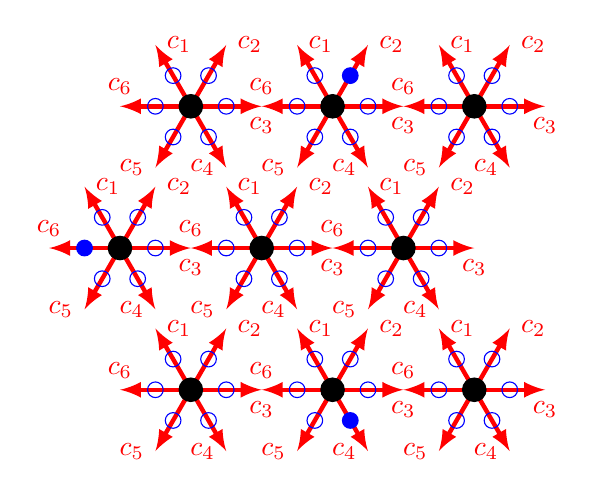
\begin{tikzpicture}[scale=0.45]
  \foreach \x in {0,4,8}
	{
	\foreach \y in {0,4,8}
		{
		\ifthenelse{\y = 4 }{
    			\coordinate (Origin) at (0 + \x - 2,0 + \y);
    			\coordinate (site1) at ({2 * cos(120) + \x- 2 }, {2 * sin(120) + \y });
    			\coordinate (site2) at ({2 * cos(60) + \x - 2}, {2 * sin(60) + \y });
    			\coordinate (site3) at ({2 * cos(0) + \x - 2}, {2 * sin(0) + \y });
    			\coordinate (site4) at ({2 * cos(-60) + \x - 2}, {2 * sin(-60) + \y });
    			\coordinate (site5) at ({2 * cos(-120) + \x - 2}, {2 * sin(-120) + \y });
    			\coordinate (site6) at ({2 * cos(-180) + \x- 2 }, {2 * sin(-180) + \y });
    
			\draw [ultra thick,-latex,red] (Origin)
        		-- (site1) node [right] {$c_1$};
    			\draw [ultra thick,-latex,red] (Origin)
        		-- (site2) node [right] {$c_2$};
    			\draw [ultra thick,-latex,red] (Origin)
        		-- (site3) node [below] {$c_3$};
    			\draw [ultra thick,-latex,red] (Origin)
        		-- (site4) node [left] {$c_4$};
    			\draw [ultra thick,-latex,red] (Origin)
        		-- (site5) node [left] {$c_5$};
    			\draw [ultra thick,-latex,red] (Origin)
        		-- (site6) node [above] {$c_6$};    
 			\coordinate (Origin) at (0 + \x- 2,0 + \y);
   			\coordinate (site1) at ({cos(120) + \x- 2 }, { sin(120) + \y });
   	 		\coordinate (site2) at ({ cos(60) + \x - 2}, { sin(60) + \y });
    			\coordinate (site3) at ({ cos(0) + \x- 2 }, { sin(0) + \y });
    			\coordinate (site4) at ({ cos(-60) + \x - 2}, { sin(-60) + \y });
    			\coordinate (site5) at ({ cos(-120) + \x - 2}, { sin(-120) + \y });
    			\coordinate (site6) at ({ cos(-180) + \x- 2 }, { sin(-180) + \y });
       		
       		\ifthenelse{\x = 0 }{
    				\node[draw,circle,inner sep=3pt,fill] at (Origin) {};
    				\node[draw,circle,inner sep=2pt,blue] at (site1) {};
    				\node[draw,circle,inner sep=2pt,blue] at (site2) {};
    				\node[draw,circle,inner sep=2pt,blue] at (site3) {};
    				\node[draw,circle,inner sep=2pt,blue] at (site4) {};
    				\node[draw,circle,inner sep=2pt,blue] at (site5) {};
    				\node[draw,circle,inner sep=2pt,fill,blue] at (site6) {};
    					
    			}%else
    			{
    				\node[draw,circle,inner sep=3pt,fill] at (Origin) {};
    				\node[draw,circle,inner sep=2pt,blue] at (site1) {};
    				\node[draw,circle,inner sep=2pt,blue] at (site2) {};
    				\node[draw,circle,inner sep=2pt,blue] at (site3) {};
    				\node[draw,circle,inner sep=2pt,blue] at (site4) {};
    				\node[draw,circle,inner sep=2pt,blue] at (site5) {};
    				\node[draw,circle,inner sep=2pt,blue] at (site6) {};
    			}
    }
    %else
    {
       	\coordinate (Origin) at (0 + \x ,0 + \y);
    		\coordinate (site1) at ({2 * cos(120) + \x }, {2 * sin(120) + \y });
    		\coordinate (site2) at ({2 * cos(60) + \x }, {2 * sin(60) + \y });
    		\coordinate (site3) at ({2 * cos(0) + \x }, {2 * sin(0) + \y });
    		\coordinate (site4) at ({2 * cos(-60) + \x }, {2 * sin(-60) + \y });
    		\coordinate (site5) at ({2 * cos(-120) + \x }, {2 * sin(-120) + \y });
    		\coordinate (site6) at ({2 * cos(-180) + \x}, {2 * sin(-180) + \y });    
		\draw [ultra thick,-latex,red] (Origin)
        -- (site1) node [right] {$c_1$};
    		\draw [ultra thick,-latex,red] (Origin)
        -- (site2) node [right] {$c_2$};
    		\draw [ultra thick,-latex,red] (Origin)
        -- (site3) node [below] {$c_3$};
    		\draw [ultra thick,-latex,red] (Origin)
        -- (site4) node [left] {$c_4$};
    		\draw [ultra thick,-latex,red] (Origin)
        -- (site5) node [left] {$c_5$};
    		\draw [ultra thick,-latex,red] (Origin)
        	-- (site6) node [above] {$c_6$};    
 		\coordinate (Origin) at (0 + \x,0 + \y);
    		\coordinate (site1) at ({cos(120) + \x }, { sin(120) + \y });
    		\coordinate (site2) at ({ cos(60) + \x }, { sin(60) + \y });
    		\coordinate (site3) at ({ cos(0) + \x}, { sin(0) + \y });
    		\coordinate (site4) at ({ cos(-60) + \x }, { sin(-60) + \y });
    		\coordinate (site5) at ({ cos(-120) + \x }, { sin(-120) + \y });
    		\coordinate (site6) at ({ cos(-180) + \x }, { sin(-180) + \y });
              		
         \ifthenelse{\x = 4 \AND \y = 0}{
    				\node[draw,circle,inner sep=3pt,fill] at (Origin) {};
    				\node[draw,circle,inner sep=2pt,blue] at (site1) {};
    				\node[draw,circle,inner sep=2pt,blue] at (site2) {};
    				\node[draw,circle,inner sep=2pt,blue] at (site3) {};
    				\node[draw,circle,inner sep=2pt,fill,blue] at (site4) {};
    				\node[draw,circle,inner sep=2pt,blue] at (site5) {};
    				\node[draw,circle,inner sep=2pt,blue] at (site6) {};
    			}%else
    			{
    				\ifthenelse{\x = 4  \AND \y = 8}{
    					\node[draw,circle,inner sep=3pt,fill] at (Origin) {};
    					\node[draw,circle,inner sep=2pt,blue] at (site1) {};
    					\node[draw,circle,inner sep=2pt,fill,blue] at (site2) {};
    					\node[draw,circle,inner sep=2pt,blue] at (site3) {};
    					\node[draw,circle,inner sep=2pt,blue] at (site4) {};
    					\node[draw,circle,inner sep=2pt,blue] at (site5) {};
    					\node[draw,circle,inner sep=2pt,blue] at (site6) {};	
    				}%else
    				{
    						\node[draw,circle,inner sep=3pt,fill] at (Origin) {};
    						\node[draw,circle,inner sep=2pt,blue] at (site1) {};
    						\node[draw,circle,inner sep=2pt,blue] at (site2) {};
    						\node[draw,circle,inner sep=2pt,blue] at (site3) {};
    						\node[draw,circle,inner sep=2pt,blue] at (site4) {};
    						\node[draw,circle,inner sep=2pt,blue] at (site5) {};
    						\node[draw,circle,inner sep=2pt,blue] at (site6) {};
    				}
    			}
    		}
    }
 }
  \end{tikzpicture}
  \caption{After propagation phase.}
        \end{block}
    \endminipage\hfill
    

	\end{frame}
	
	%six
	\section{Applications}
	\begin{frame}
	\frametitle{Applications}
	
    \begin{block}{Applications}
	\begin{itemize}
    \item Simulating rain in games.
\item Simulating rivers in games.
\item 2D fluid simulations.
\item Network congestion simulation. 
    \end{itemize}
    \end{block}
    
	\end{frame}
	
	\section{Bibliography}
	\begin{frame}
	\frametitle{Bibliography}
	
    \begin{thebibliography}{9}
\bibitem{ref1}Wolf-Gladrow, D. A. 2000. Lattice-gas cellular automata and lattice Boltzmann models. New York: Springer.
\end{thebibliography}
   
    
	\end{frame}

\end{document}
